\chapter*{Lab 5 - Texture Mapping}

In questa esercitazione si richiedeva di:
\textbf{\begin{itemize}
  \item Permettere il texture mapping 2D del toro con immagini lette da file di formato \textit{nomefile.bmp}.
  \item Permettere environment mapping sferico/cubico sfruttando il two-step mapping in modalità OpenGL.
  \item Permettere il procedural mapping basato su un procedimento algoritmico a piacere.
  \item OPZIONALE: Permettere il bump mapping dell’oggetto mesh poligonale.
\end{itemize}}

\section{Struttura}
L'applicazione è stata modificata leggermente per quanto riguarda la selezione dei diversi stadi e diversi tipi di mapping e texturing. È stata lasciata la possibilità di passare tra i tre scenari con la barra spaziatrice, ma nel caso del toro si possono selezionare le varie modalità con un menù richiamabile dal tasto destro del mouse.

Il menù presenta le seguenti possibilità di scelta:
\begin{itemize}
	\item TEXTURES, un sottomenù che contiene le varie texture che si possono associare al toro.
  \item Texture Map
  \item Environment Sphere
  \item Environment Cube
  \item Bump Map
\end{itemize}

Il menù principale e il sottomenù sono stati creati nel main e sono associati alle funzioni \texttt{menu} e \texttt{subMenuTexture} che vanno a cambiare la variabile \texttt{selectedTexture} che discrimina quale delle texture deve essere applicata nella \texttt{display}. La funzione del sottomenù fa uso della funzione \texttt{substring} per ottenere direttamente sul menù il nome della texture. Nella funzione \texttt{display}, all'interno dello scenario del toro, si sono distinti tutti i casi delle varie modalità di mapping possibile. All'interno di queste, viene principalmente effettuata l'abilitazione della texture e la \texttt{bind}. La funzione \textit{initFour} è stata modificata in modo da generare l'array che contiene tutti gli id delle texture ed è stata rinominata in \texttt{initTextures}. 

\section{Texture Map 2D}
La texture map 2D viene applicata all'interno della funzione \textit{putVert} con la \texttt{glTexCoord3f} utilizzando parametri ottenuti ragionando sul numero di texture da ripetere sul toro in orizzontale e in verticale. Il risultato è il seguente:

\begin{figure}[hbt]
    \centering
    \subfloat[Fulmine]{{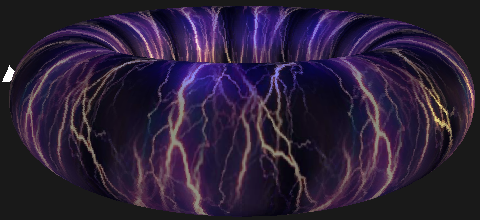
\includegraphics[height=3.7cm]{texmap1}}}
    \subfloat[Fiori]{{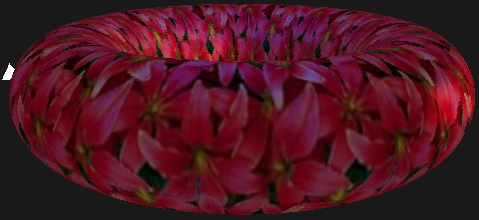
\includegraphics[height=3.7cm]{texmap2}}}\\
    \subfloat[Foglie]{{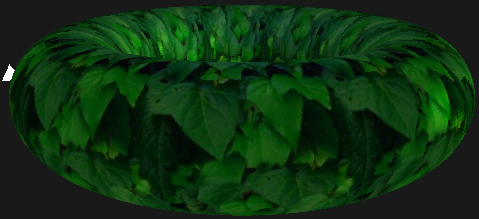
\includegraphics[height=3.7cm]{texmap3}}}
    \subfloat[Muro]{{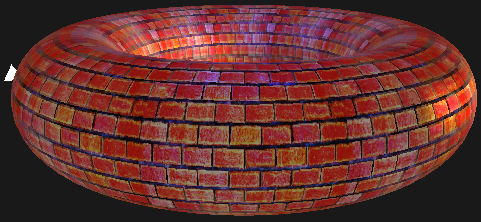
\includegraphics[height=3.7cm]{texmap4}}}\\
    \subfloat[Acqua]{{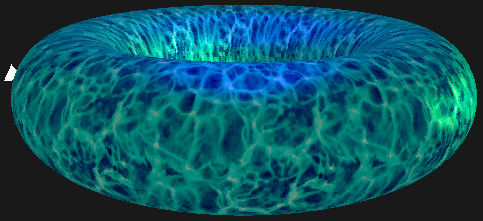
\includegraphics[height=3.7cm]{texmap5}}}
    \subfloat[Sassi]{{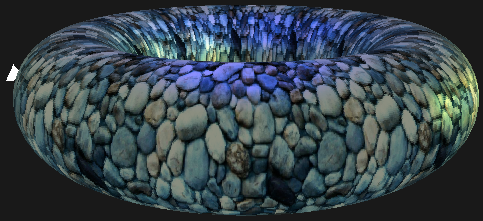
\includegraphics[height=3.7cm]{texmap6}}}
	\vspace{-0.5cm}
\end{figure}

\newpage
\section{Environment Map}
L'environment map può essere sferico o cubico. Le due modalità entrambe selezionabili dal menù: la sferica può avere due diverse texture, mentre per la cubica si è scelto di creare un solo esempio di texture per semplicità. La modalità sferica è più semplice in quanto necessita solamente di una texture già con effetto "fisheye" e di alcune funzioni che permettono il mapping sferico. La modalità cubica invece è leggermente più elaborata poichè richiede di comporre la texture dalle 6 facce del cubo come in figura:\\
 \begin{figure}[htb]
    \centering
    %\vspace{-0.7cm}
    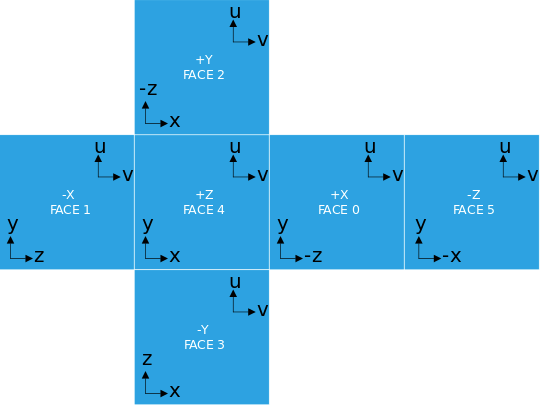
\includegraphics[width=0.7\textwidth]{cubetex}
    \caption*{\label{fig:cubetex}}
    \vspace{-0.7cm}
\end{figure}

Questa texture viene creata con la funzione \textit{initCubeMap} che inizializza nella variabile \texttt{cubeMapTexture} la texture cubica attraverso sei immagini. Il nome di quest'ultime è contenuto nell'array \texttt{cubeMap} che viene utilizzato per creare sei oggetti \texttt{RgbImage} che compongono il cubo.\\

Un esempio per ognuna delle modalità:
\begin{figure}[hbt]
    \centering
    \vspace{-0.5cm}
    \subfloat[Sphere Map]{{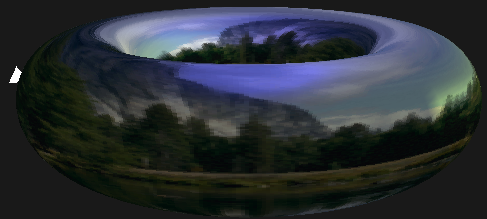
\includegraphics[height=3.5cm]{spheremap}}}
    \subfloat[Cube Map]{{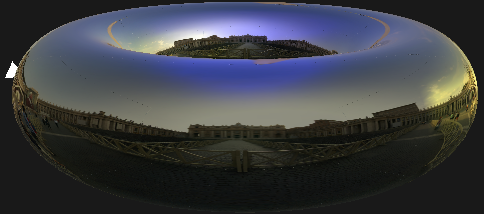
\includegraphics[height=3.5cm]{cubemap}}}
	\vspace{-0.5cm}
\end{figure}

\newpage
\section{Procedural Texture}
La texture procedurale viene creata nella funzione \texttt{initProceduralTextures} sulla base della funzione per creare la scacchiera dello scenario del cubo. Attraverso piccole variazioni dovuti a moduli e divisioni per dare diversi colori, si è ottenuto un motivo scozzese di particolare bruttezza:\\
 \begin{figure}[htb]
    \centering
    %\vspace{-0.7cm}
    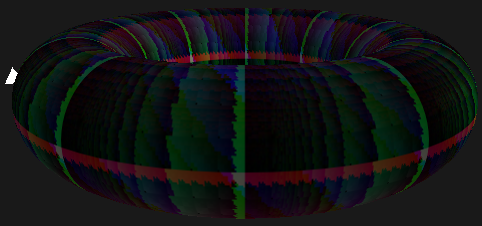
\includegraphics[width=0.8\textwidth]{procedural}
    \caption*{\label{fig:procedural}}
    %\vspace{-0.3cm}
\end{figure}

La procedurale può essere applicata sia in \textit{modalità texture map 2D}, sia in modalità \textit{environment sphere map}.


\newpage

\section{Bump Map}

no idea





















%